We investigate properties of the 1d family of 3-periodics in the Elliptic Billiard (EB). Being uniquely integrable \cite{kaloshin2018}, this object is the {\em avis rara} of planar Billiards. As a special case of Poncelet's Porism \cite{dragovic88}, it is associated with a 1d family of $N$-periodics tangent to a confocal Caustic and of constant perimeter \cite{sergei91}. Its plethora of mystifying properties has been extensively studied, see \cite{rozikov2018-billiards,stachel2016-conics} for recent treatments.

Initially we explored the loci of {\em Triangle Centers} (TCs): e.g., the Incenter $X_1$, Barycenter $X_2$, Circumcenter $X_3$, etc., see summary below. The $X_i$ notation is after  Kimberling's Encyclopedia \cite{etc}, where thousands of TCs are catalogued. Here we explore a bevy of curious behaviors displayed by the  family of 3-periodics, roughly divided into two categories (with an intermezzo):

\begin{enumerate}
    \item The {\em shape} of 3-periodics and/or TC loci: when are the former acute, obtuse, pythagorean, and the latter non-smooth, self-intersecting, non-compact? See for example this recent treatment of TCs at infinity  \cite{kimberling2020-poly-infinity}.
    \item The {\em kinematics} of EB-railed TCs: a handful of TCs\footnote{Some 50 out of 40 thousand in \cite{etc}.} is known to lie on the EB. As the family of 3-periodics is traversed, what is the nature of their motion (monotonicity, critical points, etc.). We further examine the {\em joint} motion of two EB-railed TCs which in some cases resembles a Ballet.
\end{enumerate}

In the intermezzo we introduce (i) a deceptively simple construction under which the EB bugles out the Golden Ratio, and (ii) a triangle closely related to 3-periodics\footnote{The Contact (or Intouch) Triangle of the Anticomplementary Triangle (ACT).}, whose vertices are dynamically clutched onto the EB.

Throughout the paper Figures will sometimes include a hyperlink to an animation in the format \cite[PL\#nn]{reznik2020-playlist-intriguing}, where nn is the entry into our video list on Table~\ref{tab:playlist} in Section~\ref{sec:conclusion}. Indeed, the beauty of most phenomena remain ellusive unless they are observed dynamically.

\paragraph{Related Work}

Properties of the {\em poristic} triangle family, i.e., one with fixed incircle and circumcircle, were studied in \cite{weaver1927-poristic,yiu2011-construction, odehnal2011-poristic}, where the loci of many triangle centers is described. Indeed, we noticed poristic triangles are related to the 3-periodic family by a variable similarity transform, therefore sharing with it all scale-free invariants \cite{garcia2020-poristic}.

Regarding 3-periodics, two intriguing invariants are \cite{reznik2020-intelligencer}:

\begin{enumerate}
    \item The Mittenpunkt $X_9$ is the black swan of all TCs: its locus is a {\em point} at the center of the EB\footnote{In Triangle parlance, the EB is the ``$X_9$-Centered Circumellipse''.} \cite[PL\#01]{reznik2020-playlist-intriguing}.
    \item The 3-periodic family conserves the ratio of Inradius-to-Circumradius. This implies the sum of its cosines is invariant. Suprisingly the latter holds for all $N$-periodics \cite{akopyan2020-invariants,bialy2020-invariants}.
\end{enumerate}

\noindent Other observations focused on the surprising elliptic locus of many a TC: the locus of the Incenter $X_1$ is an ellipse \cite{olga14}, as is that of the Excenters \cite{garcia2019-incenter}. The latter is similar to a rotated locus of $X_1$, see \cite[PL\#01,04]{reznik2020-playlist-intriguing}. Also elliptic are the loci of the Barycenter $X_2$ \cite{sergei2016proj}, Circumcenter $X_3$ \cite{corentin19}, Orthocenter $X_4$ \cite{garcia2019-incenter}, Center $X_5$ of the Nine-Point Circle  \cite{garcia2020-ellipses}. See \cite[PL\#05,07]{reznik2020-playlist-intriguing}. Recently we showed that out of the first 100 Kimberling Centers in \cite{etc}, exactly 29 produce elliptic loci \cite{garcia2020-ellipses}. This is quite unexpected given the non-linearities involved.

Other observations, many which find parallels in Triangle Geometry, included (i) the locus of the Feuerbach Point $X_{11}$ is on the Caustic\footnote{The Inconic centered on the Mittenpunkt $X_9$ which passes through the Extouchpoints is known as the {\em Mandart Inellipse} \cite{mw}. By definition, an Inconic is internally tangent to the sides, so it must be the Caustic.}, as is that of the Extouchpoints, though these move in opposite directions; (ii) the locus of $X_{100}$, the anticomplement of $X_{11}$, is on the EB \cite{garcia2020-new-properties}; (iii) the locus of vertices of Intouch, Medial and Feuerbach Triangles are all non-elliptic.

We still don't understand how loci ellipticity or many of the phenomena below correlate to the Trilinears of a given TC.

%\begin{figure}
%    \centering
%    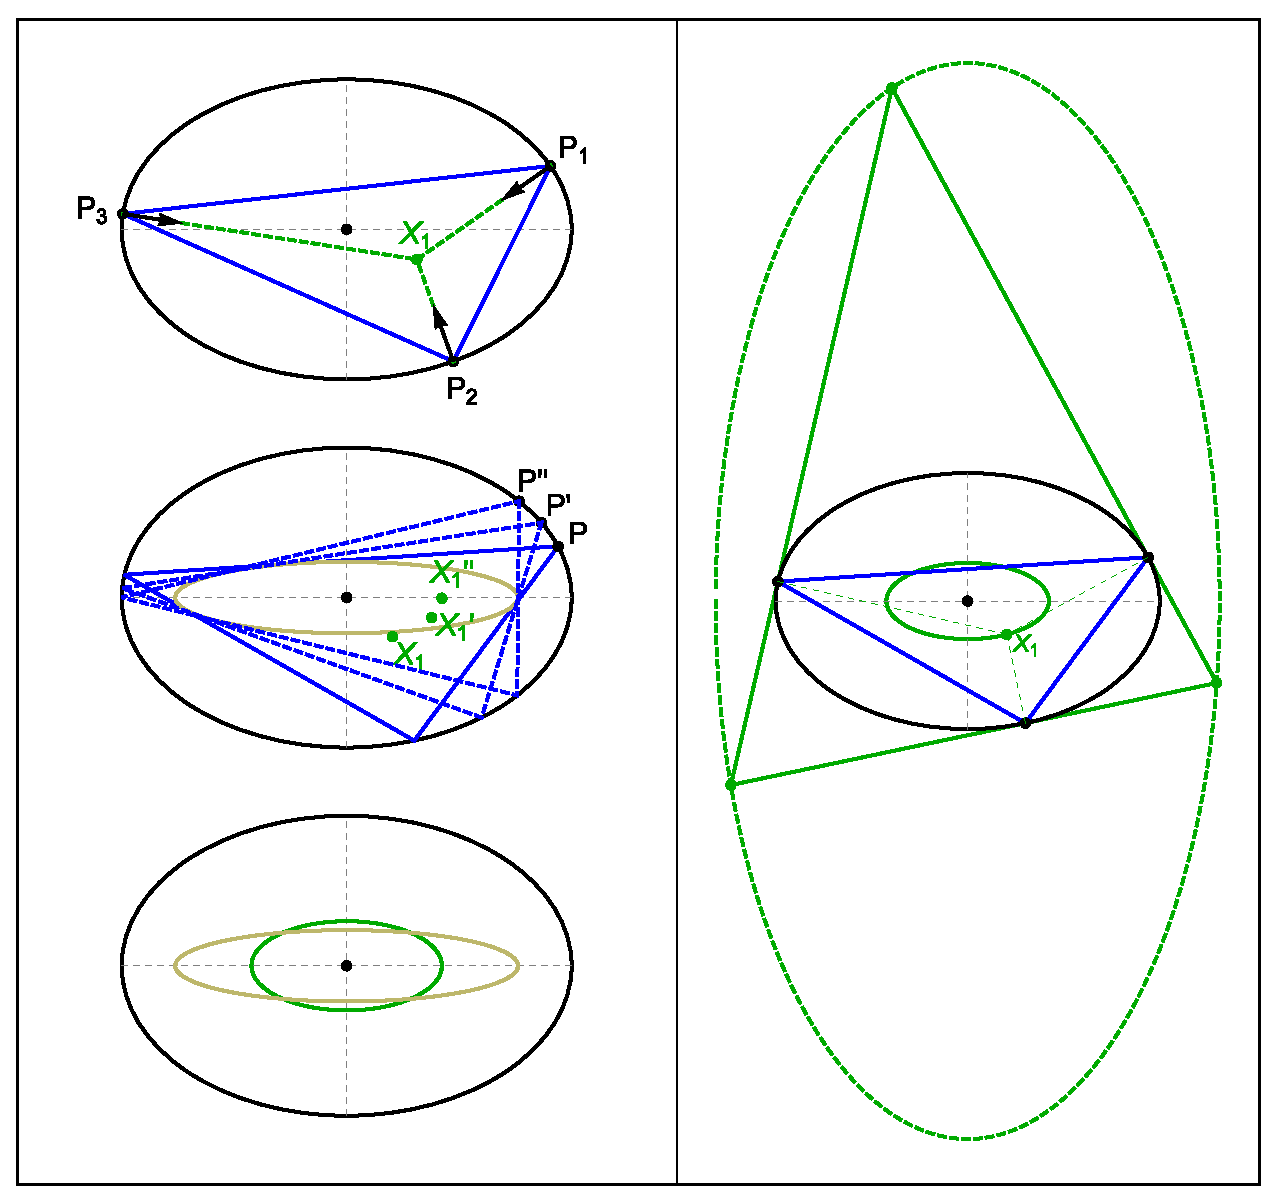
\includegraphics[width=\textwidth]{1020_pics_incenter_locus_quad.eps}
%    \caption{\textbf{Left Top}: A 3-periodic and its Incenter $X_1$: where bisectors meet. \textbf{Left Mid}: Three 3-periodics, each identified by a starting vertex $P,P',P''$, and their Incenters $X_1,X_1',X_1''$. Also shown is the  confocal Caustic (brown) which is the stationary {\em Mandart Inellipse} \cite{mw} of the 3-periodic family. \textbf{Left Bot}: the locus of $X_1$ over the 3-periodic family is an ellipse (green). Also shown is the Caustic (brown). \textbf{Right}: the Excentral Triangle (green) of a 3-periodic (blue). The locus of its vertices (the Excenters) is an ellipse (dashed green) similar to a perpendicular copy of the locus of the Incenter (solid green inside the EB). This is the stationary {\em MacBeath} Circumellipse of the Excentral Triangle \cite{mw}, centered on the latter's $X_6$ (i.e., $X_9$) \textbf{Video}:\cite[PL\#01,04]{reznik2020-playlist-intriguing}.}
%    \label{fig:incenter-loci}
%\end{figure}

%\begin{figure}
%\centering
%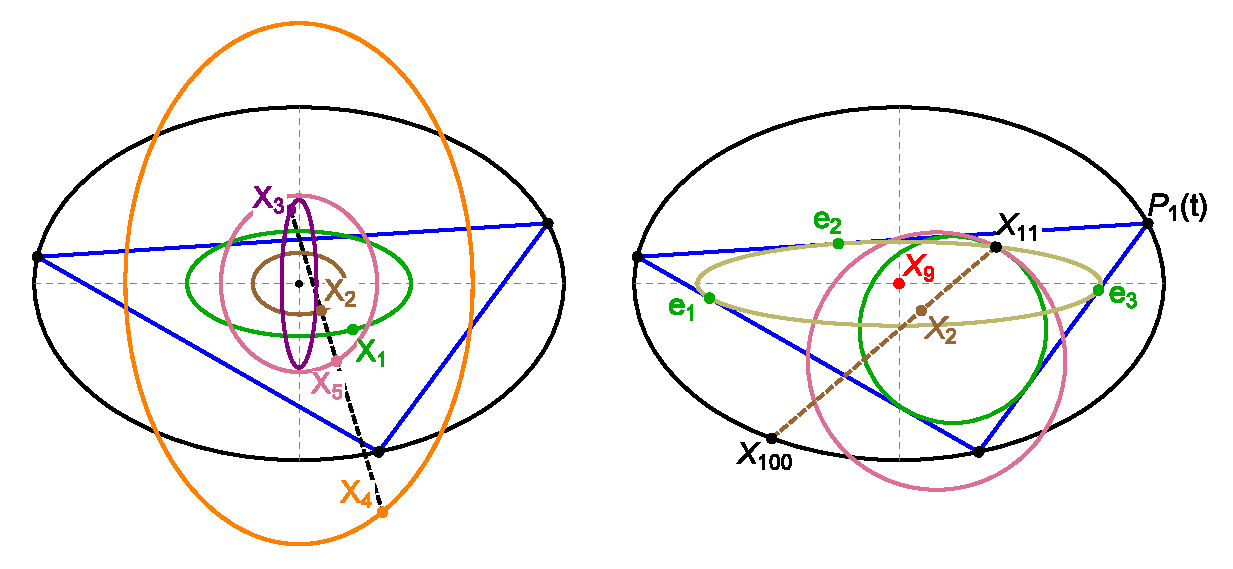
\includegraphics[width=\textwidth]{1040_pics_x12345_feuerbach_combo.eps}
%\caption{\textbf{Left}: The loci of Incenter $X_1$ (green), Barycenter $X_2$ (brown), Circumcenter $X_3$ (purple), Orthocenter $X_4$ (orange), and Center of the 9-Point Circle $X_5$ (pink), are all ellipses, \href{https://youtu.be/sMcNzcYaqtg}{Video} \cite[PL\#05]{reznik2020-playlist-intriguing}. Also shown is the {\em Euler Line} (dashed black) which for any triangle, passes through all of $X_i$, $i=1...5$ \cite{mw}. \textbf{Right}: The locus of $X_{11}$, where the Incircle (green) and 9-Point Circle (pink) meet, is the Caustic (brown), also swept (in the opposite direction) by the Extouchpoints $e_i$. $X_{100}$ (double-length reflection of $X_{11}$ about $X_2$) sweeps the EB. $X_9$ is the black swan of all points: it is stationary at the EB center \cite{reznik2020-intelligencer}. \textbf{Video:} \cite[PL\#05,07]{reznik2020-playlist-intriguing}.}
%\label{fig:x12345-feuer-combo}
%\end{figure}

%\begin{figure}
%    \centering
%    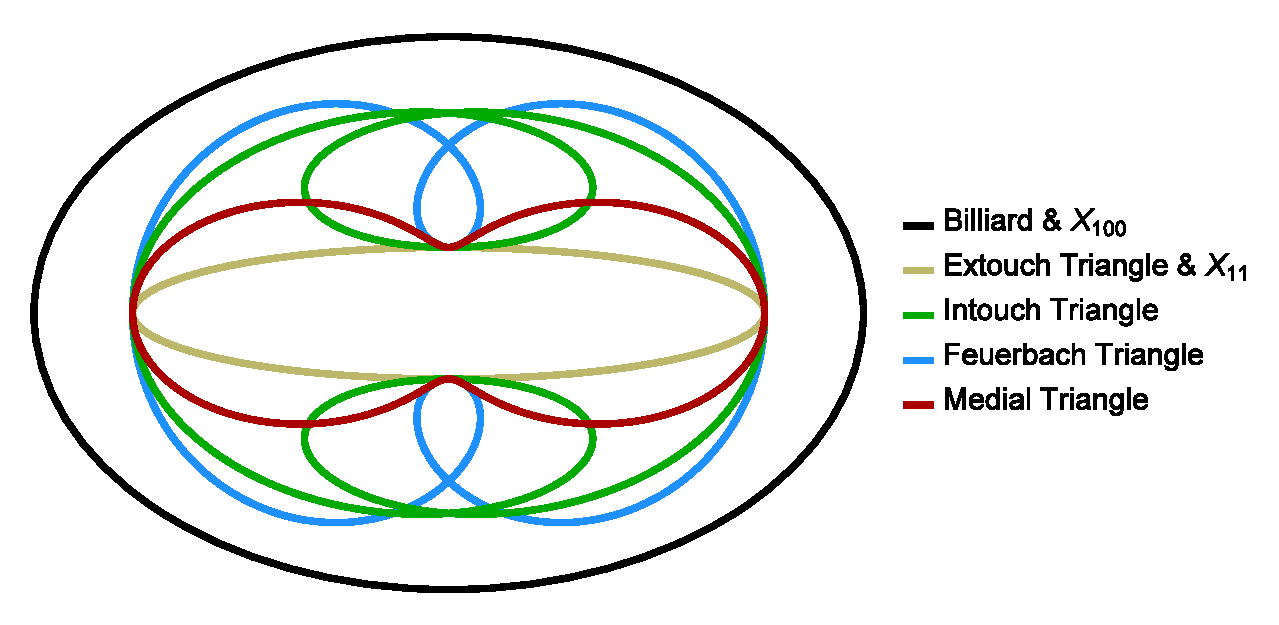
\includegraphics[width=.66\textwidth]{1050_pics_non_elliptic.eps}
%    \caption{The loci of the Intouch (green), Feuerbach (blue), and Medial (red) Triangles which are all non-elliptic. An exception is the locus of the Extouchpoints (brown), who sweep the elliptic Caustic (as does $X_{11}$ not shown). \cite[PL\#07]{reznik2020-playlist-intriguing}}
%    \label{fig:non-elliptic-vertex}
%\end{figure}
